\documentclass{article}
\usepackage{fancyhdr}
\usepackage[utf8]{inputenc}
\usepackage[english]{babel}
\usepackage{tikz, multicol, graphicx, etoolbox, enumerate, setspace, relsize, mathrsfs, verbatim}
\usepackage{amsmath, amsfonts, amssymb, amsthm, epsfig, epstopdf, titling, url, array, esvect, tikz-3dplot}
\usepackage{graphicx}
\usepackage{hyperref}
\usepackage{listings}
\usepackage{xcolor}

\hypersetup{
    colorlinks=true,
    linkcolor=blue,
    filecolor=magenta,      
    urlcolor=cyan,
    pdftitle={Overleaf Example},
    pdfpagemode=FullScreen,
    }

\definecolor{codegreen}{rgb}{0,0.6,0}
\definecolor{codegray}{rgb}{0.5,0.5,0.5}
\definecolor{codepurple}{rgb}{0.58,0,0.82}
\definecolor{backcolour}{rgb}{0.95,0.95,0.92}

\usepackage{pgfplots}
\usepackage{tcolorbox}
\usepackage{amsthm}
\usepackage{cancel}
\usepackage[left=1in,right=1in,top=1in,bottom=1in]{geometry}
\usepackage[tableaux]{prooftrees}

\lstdefinestyle{mystyle}{
    backgroundcolor=\color{backcolour},   
    commentstyle=\color{codegreen},
    keywordstyle=\color{magenta},
    numberstyle=\tiny\color{codegray},
    stringstyle=\color{codepurple},
    basicstyle=\ttfamily\footnotesize,
    breakatwhitespace=false,         
    breaklines=true,                 
    captionpos=b,                    
    keepspaces=true,                 
    numbers=left,                    
    numbersep=5pt,                  
    showspaces=false,                
    showstringspaces=false,
    showtabs=false,                  
    tabsize=2
}

\lstset{style=mystyle}

\pagestyle{fancy}
\fancyhf{}
\fancyhead[L,RO]{Tasksheet 10}
\fancyhead[R,RO]{Fundamentals of Computational Mathematics}
\fancyfoot[L,RO]{Xiang Gao}
\fancyfoot[R,RO]{Math 4610}
\renewcommand{\headrulewidth}{0.4pt}% Default \headrulewidth is 0.4pt
\renewcommand{\footrulewidth}{0.4pt}% Default \footrulewidth is 0pt
\def\checkmark{\tikz\fill[scale=0.4](0,.35) -- (.25,0) -- (1,.7) -- (.25,.15) -- cycle;} 

\begin{document}

\section*{Task 1}
I have created the following code that implement the power method for finding the eigenvalue of largest magnitude. The code is documented \href{https://github.com/GoByMark/math4610/blob/main/Homework_Tasks/Tasksheet_10/src/powerMethod.py}{here} in the \href{https://github.com/GoByMark/math4610/blob/main/Homework_Tasks/Software_Manual/Software_Manual_toc.md}{Software Manual}.
\lstinputlisting[language=Python]{powerMethod.py}

\newpage

with the following output:
\begin{center}
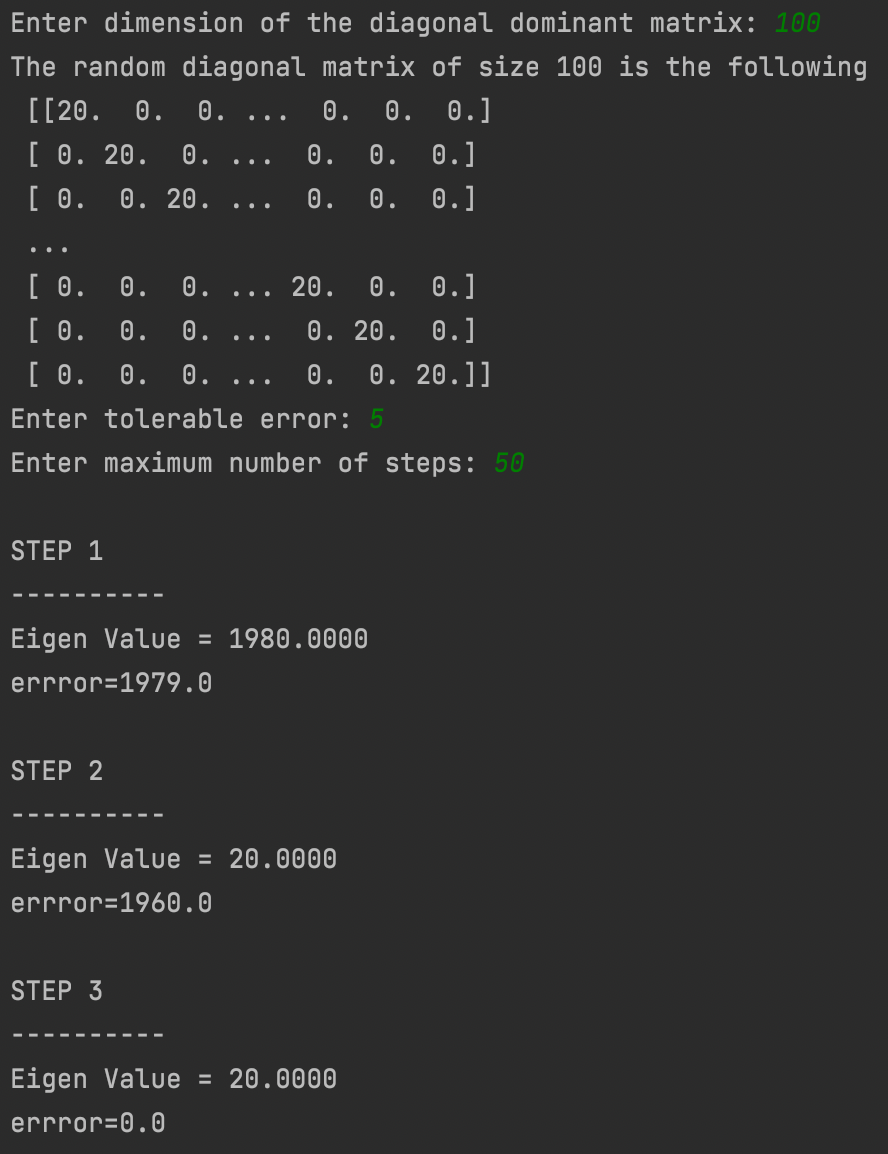
\includegraphics[width=\textwidth]{Screenshots/1.png}\\
{\bf Figure 1.} Running the powerMethod.py From the IDE.
\end{center}

\newpage

\section*{Task 2}
I have created the following code that implement the power method for finding the eigenvalue of smallest magnitude. The code is documented \href{https://github.com/GoByMark/math4610/blob/main/Homework_Tasks/Tasksheet_10/src/invPowerMethod.py}{here} in the \href{https://github.com/GoByMark/math4610/blob/main/Homework_Tasks/Software_Manual/Software_Manual_toc.md}{Software Manual}.
\lstinputlisting[language=Python]{invPowerMethod.py}

\newpage

with the following output:
\begin{center}
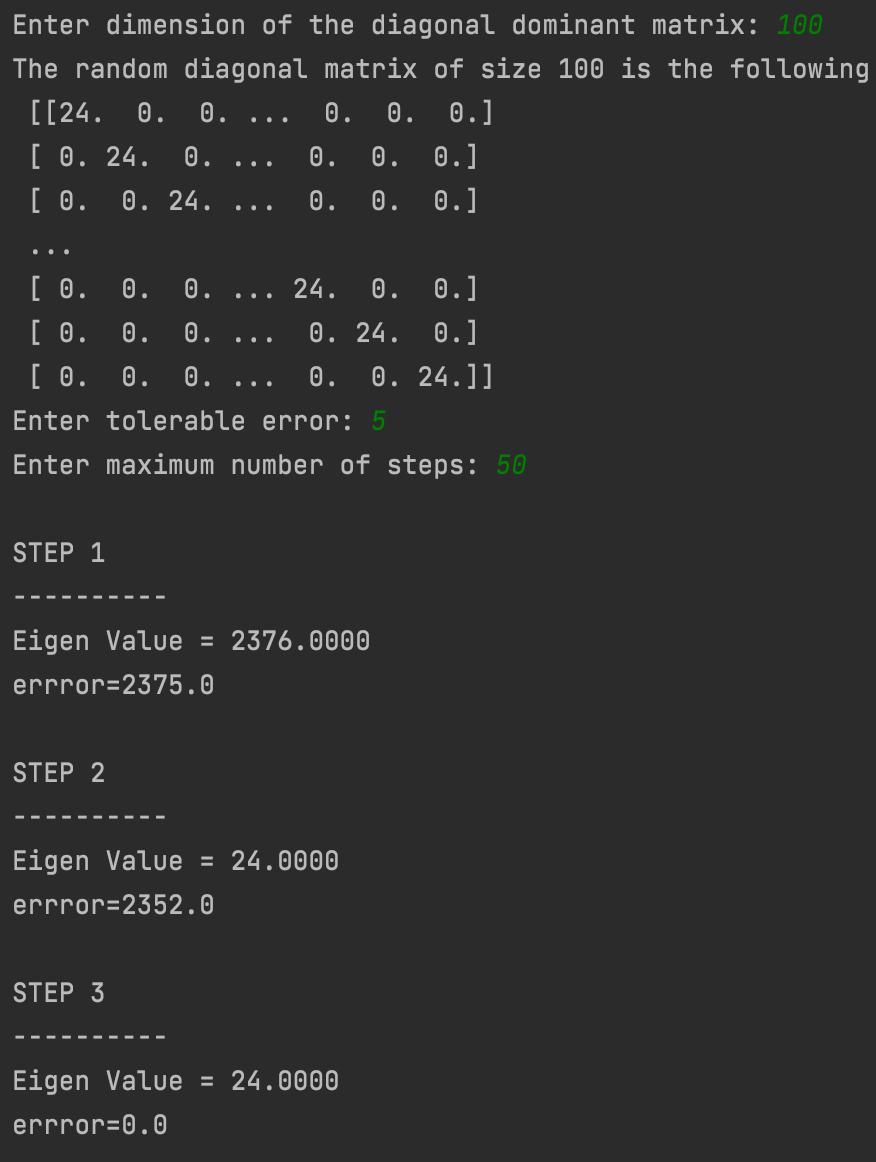
\includegraphics[width=0.8\textwidth]{Screenshots/2.png}\\
{\bf Figure 2.} Running the invPowerMethod.py From the IDE.
\end{center}

\newpage

\section*{Task 3}
I have created the following routine that compute the 1-matrix norm for a square matrix. The routine is documented \href{https://github.com/GoByMark/math4610/blob/main/Homework_Tasks/Tasksheet_10/src/mat1Norm.py}{here} in the \href{https://github.com/GoByMark/math4610/blob/main/Homework_Tasks/Software_Manual/Software_Manual_toc.md}{Software Manual}.
\lstinputlisting[language=Python]{mat1Norm.py}
I have also created the following testing routine for the 1-matrix norm
\lstinputlisting[language=Python]{Task_3.py}
with the following output:
\begin{center}
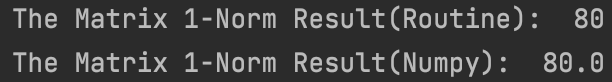
\includegraphics[width=\textwidth]{Screenshots/3.png}\\
{\bf Figure 3.} Testing the Routine with Numpy.
\end{center}

\section*{Task 4}
I have created the following routine that compute the $\infty$-matrix norm for a square matrix. The routine is documented \href{https://github.com/GoByMark/math4610/blob/main/Homework_Tasks/Tasksheet_10/src/matInfNorm.py}{here} in the \href{https://github.com/GoByMark/math4610/blob/main/Homework_Tasks/Software_Manual/Software_Manual_toc.md}{Software Manual}.
\lstinputlisting[language=Python]{matInfNorm.py}
I have also created the following testing routine for the $\infty$-matrix norm
\lstinputlisting[language=Python]{Task_4.py}
with the following output:
\begin{center}
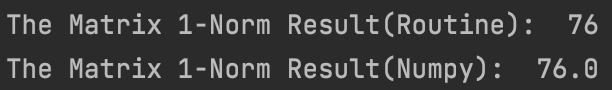
\includegraphics[width=\textwidth]{Screenshots/4.png}\\
{\bf Figure 4.} Testing the Routine with Numpy.
\end{center}

\section*{Task 5}
Before jumping on to this task, I have realized my Power Method is not sufficient enough, so I have updated my power method and inverse method routine into the following, they are all documented in the \href{https://github.com/GoByMark/math4610/blob/main/Homework_Tasks/Software_Manual/Software_Manual_toc.md}{Software Manual}.
\lstinputlisting[language=Python]{newPowerMethodRoutine.py}
\lstinputlisting[language=Python]{newInversePowerRoutine.py}
Hence, the following is the routine for computing the condition number, it is documented \href{https://github.com/GoByMark/math4610/blob/main/Homework_Tasks/Tasksheet_10/src/conNum.py}{here} in the \href{https://github.com/GoByMark/math4610/blob/main/Homework_Tasks/Software_Manual/Software_Manual_toc.md}{Software Manual}.
\lstinputlisting[language=Python]{conNum.py}
which has the following output:
\begin{center}
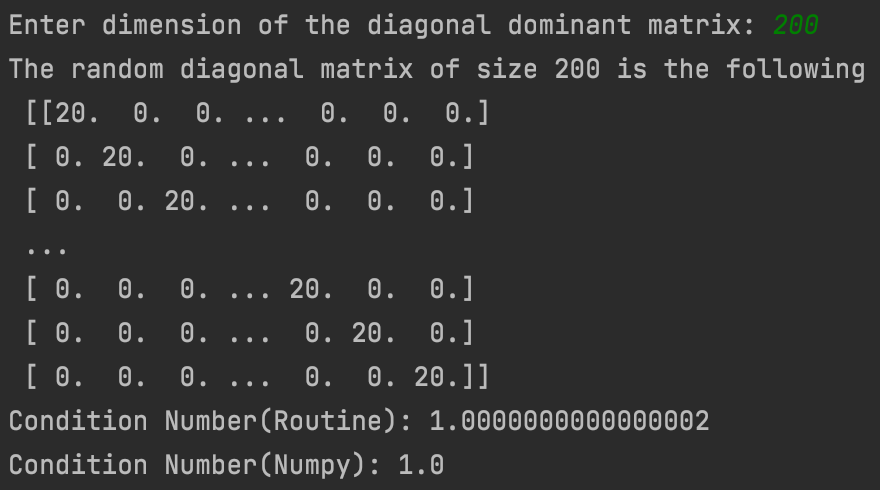
\includegraphics[width=\textwidth]{Screenshots/5.png}\\
{\bf Figure 5.} Testing the Routine with Numpy.
\end{center}

\section*{Task 6}
\href{https://github.com/GoByMark/math4610/blob/main/Homework_Tasks/Software_Manual/Software_Manual_toc.md}{Please click here to access the Software Manual}.

\end{document}